\subsection{Development Board}

The development board for this project is the Raspberry Pi 4 Model B \ref{fig:rasp}, considering it is one of the constraints identified in the analysis phase ([ref]). This board includes a 64-bit quad-core ARM processor, the BCM2711, multimedia and connection features, ressembling to a computer-like board that serves multiple applications. The following list show the Raspberry Pi 4 Model B main features:

\begin{itemize}
        \item 2GB LPDDR4-3200 SDRAM;
        \item 2.4 GHz and 5.0 GHz IEEE 802.11ac wireless, Bluetooth 5.0, BLE;
        \item Raspberry Pi standard 40 pin GPIO header;   
        \item 2 USB 3.0 ports and 2 USB 2.0 ports;
        \item 2 micro-HDMI ports;
        \item 1 display port (2-lane MIPI DSI);
        \item 1 camera port (2-lane MIPI CSI);
        \item 1 jack 3,5 mm port (4-pole stereo audio and composite video port);
		\item graphic support (OpenGL ES 3.1, Vulkan 1.0);
		\item Micro-SD card slot.
\end{itemize}

%\item Raspberry Pi standard 40 pin GPIO header (fully backwards compatible with previous boards)

\begin{figure}[ht]
	\centering
	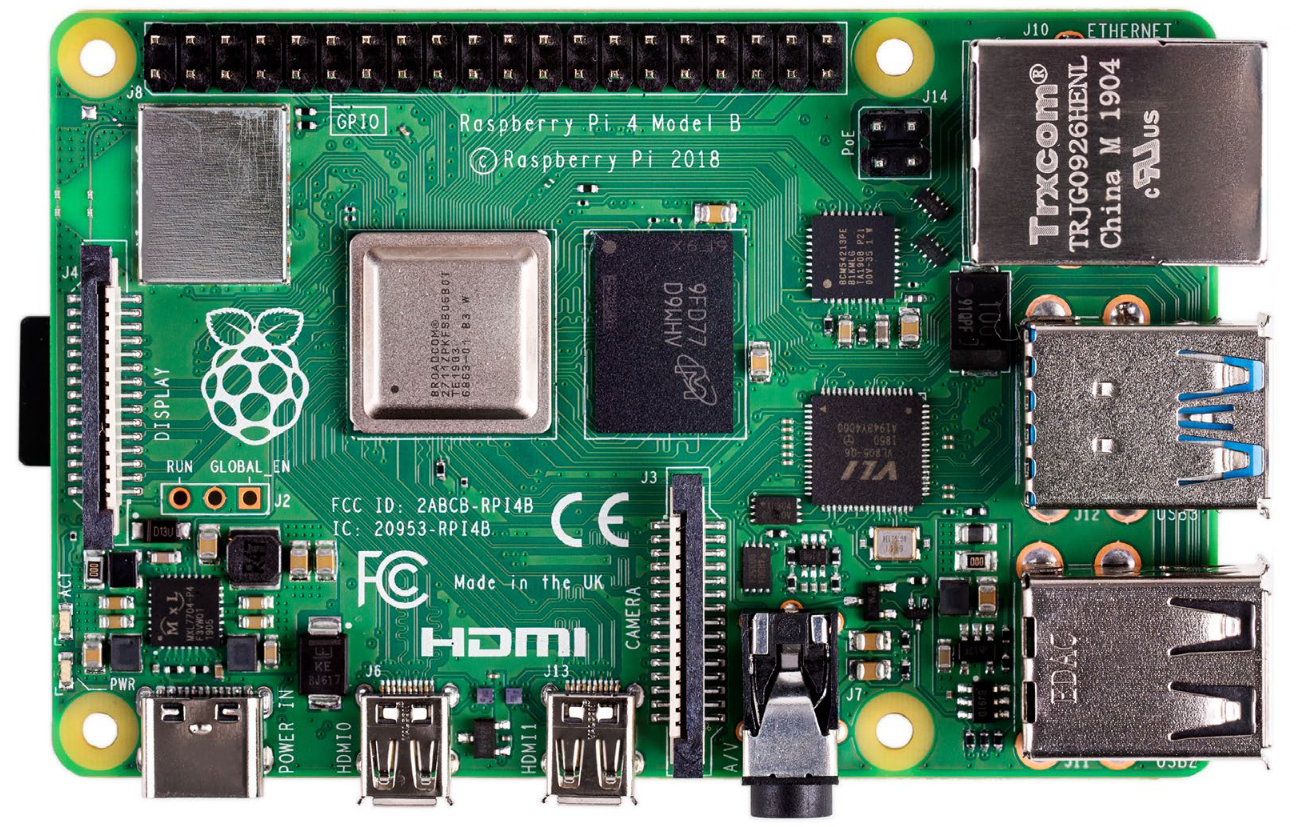
\includegraphics[width=.75\textwidth]{raspberryPi}
	\caption{Raspberry Pi 4 Model B.}
	\label{fig:rasp}
\end{figure}

\subsubsection{\ac{gpio}}

The Raspberry Pi 4 Model B board comes with a standard 40 pin GPIO header, that allows to interface with external peripherals. This GPIO also provides some interface technologys, like UART, I2C or SPI. The GPIO pinout of this board is shown in figure \ref{fig:rasp_pinout} \cite{pinout}.

\begin{figure}[ht]
	\centering
	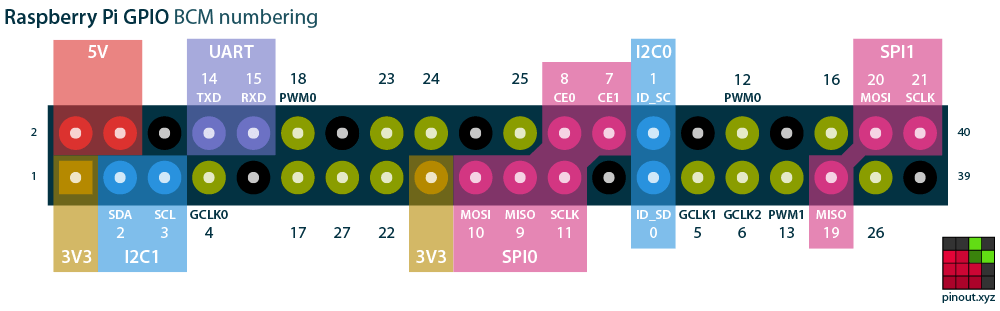
\includegraphics[width=1\textwidth]{raspberryPi_pinout}
	\caption{Raspberry Pi 4 Model B GPIO Pinout.}
	\label{fig:rasp_pinout}
\end{figure}